\section{Fazit} \label{fazit}

Den Ergebnissen aus Kapitel \ref{evaluation} ist zu entnehmen, dass es, in Hinblick auf die verwendeten Vergleichdaten, bei vermeintlich besserem Wetter mehr Ufo-Sichtungen gemeldet werden als bei schlechterem Wetter. Da allerdings nur für eine sehr geringe Anzahl an Ufo-Sichtungen dazu passende Wetterdaten gefunden wurden, lässt sich die Aussagekraft der Ergebnisse nicht als endgültiges Ergebnis festlegen, sondern kann als Wegweiser für weitere Forschungen dienen. Eine weiterführende Herangehensweise wäre zum Beispiel die Betrachtung Wetterdaten von anderen Anbietern. Für Forschungen, welche außerhalb der Wetterzusammenhänge liegen, erweisen sich Uhrzeit der Sichtung (Morning Morality Effekt) sowie die Frage, ob es in der Nähe von Weltraumbahnhöfen, militärischen Einrichtungen oder Flughäfen zu überdurchschnittlich vielen Sichtungen kommt, als interessant. Ob es sich bei den vermeintlichen Ufo-Sichtungen wirklich um Ufos handelt, oder diese \enquote{Sichtungen} nur Verwechselungen mit anderen Flugobjekten oder bewusste Fehlinformationen sind, können allein durch die verwendeten Daten nicht belegt werden.

\begin{figure}[t]
    \centering
    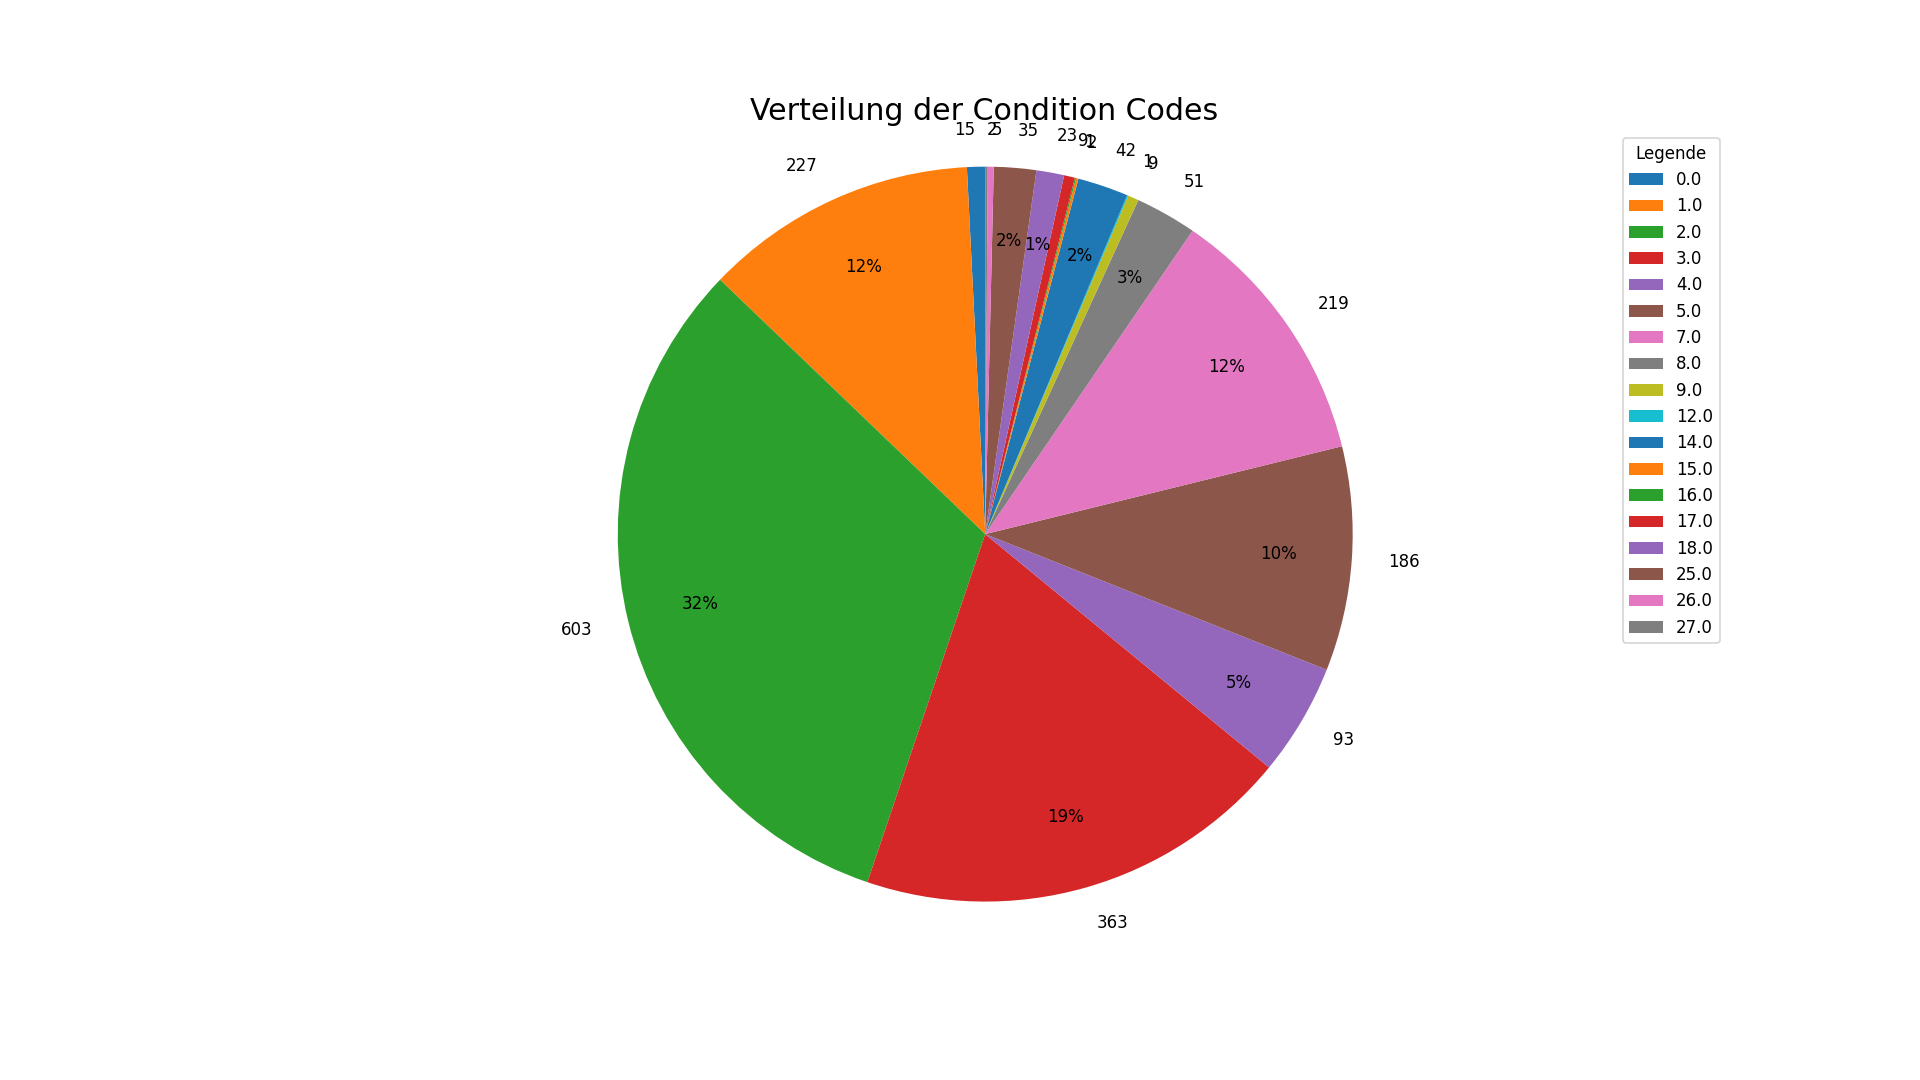
\includegraphics[width=\columnwidth]{condition_codes_pie.png}
    \caption{Verteilung der Condition Codes.}
    \label{fig:coco_pie}
\end{figure}